% Module 4 section file. Included by ../module4_alfven_continuum_eigenmodes.tex.
\section{Baseline case, numerical results, and physical interpretation}
\label{sec:baseline_results}

\subsection{Version-controlled input parameters}
The baseline case is stored in byte-identical JSON files in the Python and MATLAB case directories. Table~\ref{tab:baseline_parameters_textbook} lists the mathematical inputs.

\begin{table}[htbp]
\centering
\begin{tabular}{lll}
\toprule
Quantity & Symbol & Baseline value\\
\midrule
Reference major radius & $R_0$ & \SI{3.0}{m}\\
Minor-radius metadata & $a$ & \SI{1.0}{m}\\
Reference magnetic field & $B_0$ & \SI{2.5}{T}\\
Axis mass density & $\rho_0$ & $3.3\times10^{-8}\ \mathrm{kg\,m^{-3}}$\\
Edge density fraction & $f_\rho$ & 0.20\\
Density exponent & $a_\rho$ & 2\\
Axis transform & $\iota_0$ & 0.35\\
Edge transform & $\iota_1$ & 0.65\\
Transform exponent & $a_\iota$ & 1\\
Toroidal mode number & $n$ & 2\\
Poloidal harmonics & $(m,m+1)$ & $(3,4)$\\
Coupling fraction & $\epsilon_c$ & 0.45\\
Coupling width & $w_c$ & 0.22\\
Radial stiffness fraction & $\epsilon_r$ & 0.0015\\
Radial cells & $N$ & 256\\
Requested eigenpairs & $k$ & 8\\
\bottomrule
\end{tabular}
\caption{Version-controlled parameters for the reduced Alfv\'en-eigenmode benchmark. The listed minor radius is metadata and does not enter the current normalized radial operator.}
\label{tab:baseline_parameters_textbook}
\end{table}

\subsection{Crossing calculation}
For $n=2$ and $m=3$,
\begin{equation}
\iota_c=\frac{2n}{2m+1}=\frac{4}{7}=0.5714286.
\end{equation}
Because the transform profile is linear,
\begin{equation}
s_c=\frac{\iota_c-\iota_0}{\iota_1-\iota_0}
=\frac{0.5714286-0.35}{0.65-0.35}
=0.7380952.
\end{equation}
For $N=256$, the nearest cell center is
\begin{equation}
s_{188}=\left(188+\frac{1}{2}\right)\frac{1}{256}=0.736328125.
\end{equation}
The gap values stored in metadata are evaluated at this nearest center rather than at an interpolated exact $s_c$.

\subsection{Alfv\'en-speed variation}
At the first cell center, the baseline Alfv\'en speed is approximately
\begin{equation}
v_A\approx1.228\times10^7\ \mathrm{m\,s^{-1}}.
\end{equation}
Near the crossing it is approximately
\begin{equation}
v_A(s_c)\approx1.631\times10^7\ \mathrm{m\,s^{-1}},
\end{equation}
and near the final cell center it is approximately
\begin{equation}
v_A\approx2.724\times10^7\ \mathrm{m\,s^{-1}}.
\end{equation}
The increase is caused by the outward decrease in density. This variation significantly bends the continuum branches and shows why a single constant-$v_A$ estimate is only an order-of-magnitude guide.

\subsection{Local continuum and avoided crossing}
Figure~\ref{fig:continuum_textbook} shows the uncoupled branches and the local eigenvalues of the coupled $2\times2$ matrix.

\begin{figure}[htbp]
\centering
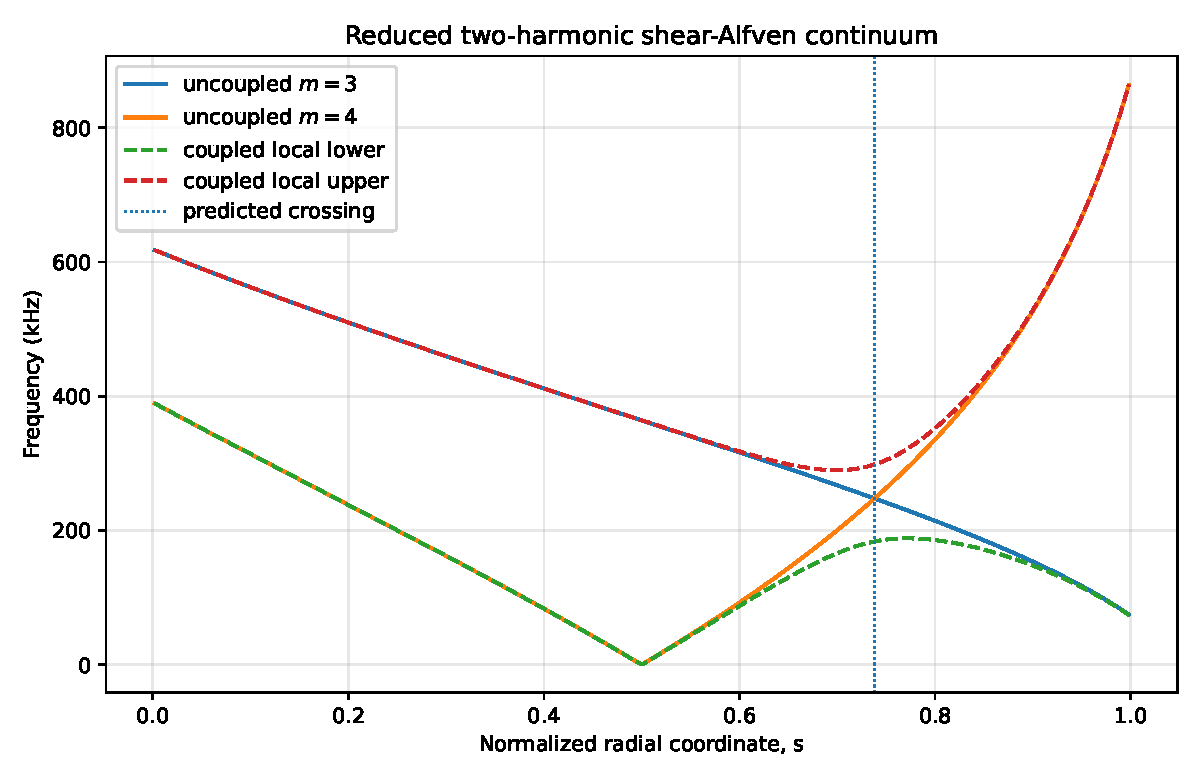
\includegraphics[width=0.88\textwidth]{figures/module4_reduced_ae_continuum.pdf}
\caption{Baseline uncoupled continuum branches and local coupled branches. The vertical line is the analytic neighboring-harmonic crossing coordinate. Frequencies are local functions of radius, not global eigenvalues.}
\label{fig:continuum_textbook}
\end{figure}

At the nearest cell center to $s_c$, the local lower and upper coupled frequencies are
\begin{equation}
f_-=\SI{183.207}{kHz},
\qquad
f_+=\SI{297.516}{kHz}.
\label{eq:baseline_gap_interval}
\end{equation}
The interval between them is a local avoided-crossing interval. It is not automatically a global gap over all radii.

\subsection{Computed global eigenfrequencies}
The frozen Python reference eigenpairs are listed in Table~\ref{tab:baseline_eigenpairs_textbook}.

\begin{table}[htbp]
\centering
\begin{tabular}{r r r}
\toprule
Mode index & Frequency (kHz) & Relative algebraic residual\\
\midrule
1 & 160.504376 & $1.38\times10^{-11}$\\
2 & 271.117830 & $6.41\times10^{-12}$\\
3 & 323.043576 & $3.99\times10^{-12}$\\
4 & 358.050072 & $5.24\times10^{-12}$\\
5 & 419.201855 & $3.25\times10^{-12}$\\
6 & 433.809373 & $4.69\times10^{-12}$\\
7 & 498.246555 & $2.90\times10^{-12}$\\
8 & 508.475762 & $2.42\times10^{-12}$\\
\bottomrule
\end{tabular}
\caption{Baseline 256-cell eigenpairs. Residuals use Eq.~\eqref{eq:relative_eigen_residual}.}
\label{tab:baseline_eigenpairs_textbook}
\end{table}

Mode 2 has frequency $\SI{271.118}{kHz}$, which lies inside the local interval in Eq.~\eqref{eq:baseline_gap_interval}. That is why it is selected for the existing representative-mode figure.

\subsection{Harmonic weights and radial localization}
For a normalized mode, define harmonic weights
\begin{align}
W_m&=\int_0^1\xi_m^2ds,\\
W_{m+1}&=\int_0^1\xi_{m+1}^2ds,
\end{align}
so $W_m+W_{m+1}=1$. Define the radial probability-like density
\begin{equation}
P(s)=\xi_m^2(s)+\xi_{m+1}^2(s).
\end{equation}
Although $P$ is not a quantum probability, its normalized integral makes it useful for reporting a centroid and spread:
\begin{align}
\bar s&=\int_0^1sP(s)ds,\\
\sigma_s&=\left[\int_0^1(s-\bar s)^2P(s)ds\right]^{1/2}.
\end{align}
Diagnostics computed directly from the frozen eigenmode CSV are shown in Table~\ref{tab:harmonic_diagnostics}.

\begin{table}[htbp]
\centering
\small
\begin{tabular}{r r r r r r}
\toprule
Mode & $W_{m=3}$ & $W_{m=4}$ & Peak $s$ & $\bar s$ & $\sigma_s$\\
\midrule
1 & 0.0069 & 0.9931 & 0.4707 & 0.4696 & 0.1258\\
2 & 0.0796 & 0.9204 & 0.2754 & 0.4294 & 0.2238\\
3 & 0.6991 & 0.3009 & 0.7324 & 0.5849 & 0.2424\\
4 & 0.1886 & 0.8114 & 0.0840 & 0.3829 & 0.2753\\
5 & 0.3089 & 0.6911 & 0.0020 & 0.4239 & 0.2581\\
6 & 0.6980 & 0.3020 & 0.4746 & 0.5018 & 0.2352\\
7 & 0.4533 & 0.5467 & 0.3730 & 0.4307 & 0.2485\\
8 & 0.5579 & 0.4421 & 0.3574 & 0.4364 & 0.2544\\
\bottomrule
\end{tabular}
\caption{Harmonic and localization diagnostics evaluated from the version-controlled 256-cell eigenvectors.}
\label{tab:harmonic_diagnostics}
\end{table}

\subsection{What the representative mode actually demonstrates}
Figure~\ref{fig:eigenmode_textbook} shows mode 2.

\begin{figure}[htbp]
\centering
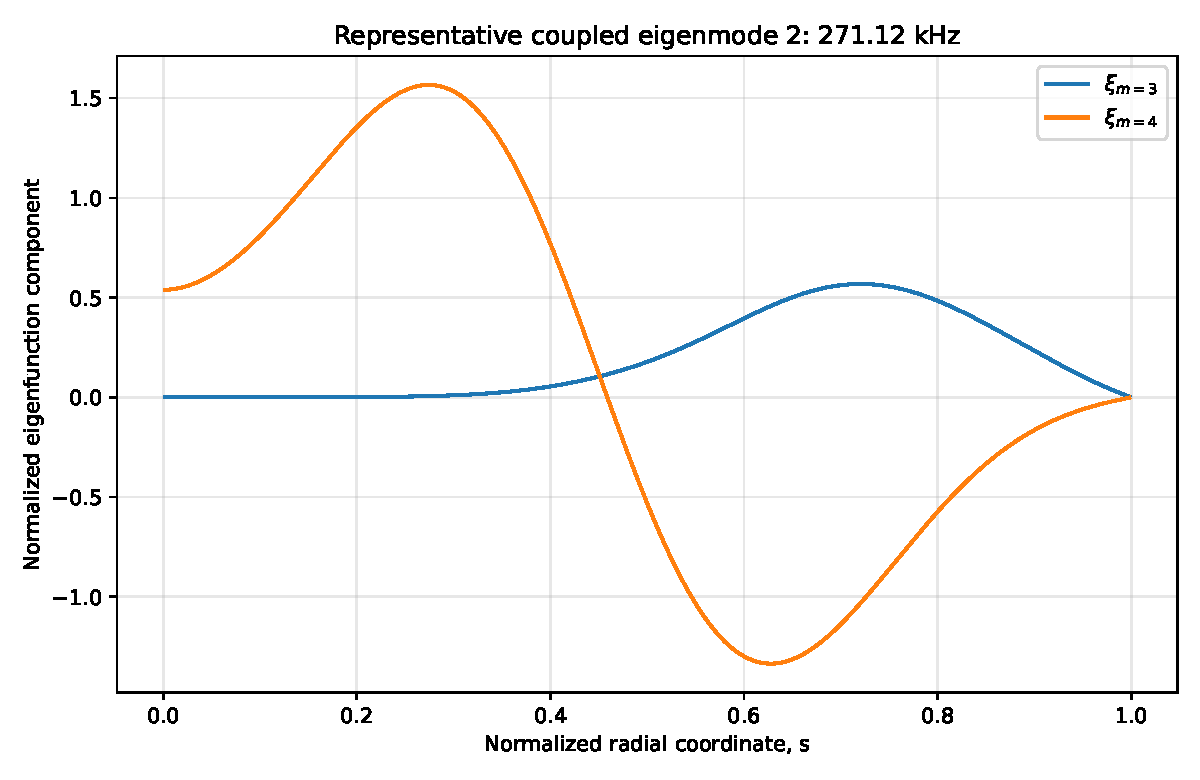
\includegraphics[width=0.86\textwidth]{figures/module4_reduced_ae_eigenmode.pdf}
\caption{Two harmonic components of mode 2, selected because its frequency is nearest the center of the local avoided-crossing interval. The mode is normalized by Eq.~\eqref{eq:benchmark_normalization}.}
\label{fig:eigenmode_textbook}
\end{figure}

The quantitative diagnostics require a careful interpretation:
\begin{itemize}[leftmargin=1.6em]
\item Mode 2 is predominantly the $m=4$ component, with $W_{m=4}\approx0.920$.
\item Its peak amplitude occurs at $s\approx0.275$, not at the analytic crossing $s_c\approx0.738$.
\item Its radial spread is broad, $\sigma_s\approx0.224$.
\item Mode 3 peaks close to $s_c$ and is more mixed, but its frequency $\SI{323.044}{kHz}$ is above the local upper branch value at the crossing cell.
\end{itemize}
Therefore, the baseline robustly demonstrates a coupled self-adjoint eigenproblem, an avoided crossing, mixed global eigenfunctions, and convergent discrete frequencies. It does \emph{not} yet demonstrate a strongly trapped, crossing-centered, realistic TAE. Calling the model a \emph{reduced coupled-harmonic benchmark with a TAE-like avoided crossing} is accurate. Calling mode 2 a validated stellarator TAE would be an overstatement.

\subsection{Why this honest limitation is useful}
A verification benchmark need not reproduce every desired physical feature. In fact, the mismatch between a local-gap frequency criterion and actual eigenfunction localization is pedagogically valuable. It shows why mode classification must use spatial structure and parameter continuation, not frequency alone. A future benchmark revision can deliberately tune $D(s)$, coupling width, profiles, or boundary conditions to generate a more clearly localized gap mode while retaining the current case as a frozen regression target.
